
\documentclass[11pt]{article}
\usepackage[margin = 1in]{geometry}
\usepackage[none]{hyphenat}
\usepackage{fancyhdr}
\usepackage{graphicx}
\graphicspath{{./images/}}
\usepackage{float}



\pagestyle{fancy}
\fancyhead{}
\fancyfoot{}
\fancyhead[L]{\slshape \MakeUppercase{Term Project}}
\fancyhead[R]{\slshape Mason Edmison}
\fancyfoot[C]{\thepage}

%%%%
% hack to remove indent
\newlength\tindent
\setlength{\tindent}{\parindent}
\setlength{\parindent}{0pt}
\renewcommand{\indent}{\hspace*{\tindent}}
%%%%

\begin{document}

\begin{titlepage}
\begin{center}
\Large{\textbf{Term Project}} \\
\Large{\textbf{CS 710 - Artificial Intelligence}} \\

\vfill
\line(1,0){400} \\

\Large{\textbf{Coreference Resolution in Biomedical Text:}} \\
\Large{\textbf{Improving Performance with Ontologies and Domain Specific NER}} \\

\line(1,0){400}\\
\vfill
Mason Edmison\\
University of Wisconsin-Milwaukee\\
12/10/2019
\end{center}
\end{titlepage}

\section{Introduction}
For my final project, I built a biomedical coreference resolution system using python open source libraries. Coreference Resolution is hard and important problem as there are many applications that could benefit or have benefited from coreference resolution. Some of those applications are: question answering, text summarization, information extraction, and machine translation.

\section{Recent Work}

\subsection{Coreference}
Corefence resolution is a classical natural language processing problem where the task is to indentify which mentions in a text refer to the same real-world entity. 

\begin{figure}[h]
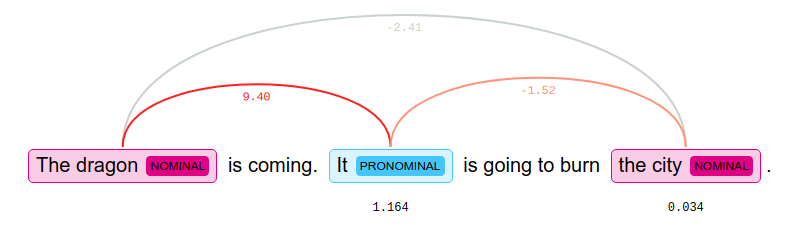
\includegraphics[width=8cm]{coref_vis}
\centering
\caption{Example of resolving coferring expression \textit{it} to antecedent {dragon}}
\end{figure}

To better isolate specific sub-tasks, it is helpful to think of the reference the generic algorithm for anaphora and coreference resolution proposed by Ng et al., 2002. Algorithms and techniques decribed later in the paper will focus on certain sub-tasks to improve the performance of cluster detection. 
\begin{enumerate}
\item \textbf{Identification of referring expressions} Identify all noun phrases in the text. 
\item \textbf{Characterization of referring expressions} Composed of two sub-tasks: first, define a representation of a discourse entity. This representation determines the knowledge regarding a discourse entity that the algorithm needs in order to perform the remaining steps. Second, compute the information specified in the representation for each entity. 
\item \textbf{Anaphoricity determination} Determine whether a discourse entity is anaphoric or not. Non-anaphophoric entities, do not posses an antecedent and that algorithm will not search for these entitites. 
\item \textbf{Generation of antecedent candidates} Once a NP is determined to be anaphoric, the algorithm indentifies scope of the NP and gathers those NPs that falling with its scope to generate a list of canidate antecedents for it.
\item \textbf{Filtering} Remove unreasonable canidate antecedents for each anaphoric noun phrase. Can be based off of a set of rules or hard constraints. This step reduces the amount of processing that needs to be performed by the algorithm.
\item \textbf{Scoring/ Ranking} Score that indicates the likelihood that two NPs co-specify.
\item \textbf{Searching/ Clustering} Select an antecedent for a given anaphor from the list of canidate antecendnts returned by the previous step. If this list is empty then no antecedent will be selected for this anaphor. 
\end{enumerate}


\subsection{Neural Network Systems}
Since this task requires knowledge at all levels of language processing, including lexical, syntactic, semantic, and world knowledge, success in this problem is indicative of advancement of language technologies. Appropriately, due to advancements in computational power and reinforcement learning, coreference resolution has experienced a revival of sorts with many performant systems proposed in recent times. More specifically, Neural Network based coreference systems employing entity-level information and reinforcement learning have produced new scores outperforming the previous state-of-the-art. An example of such a system is the Deep Reinforcement Learning model proposed by Clark and Manning, 2016.

Specifically, this system is a deep neural network that learns distributed representations of coreference clusters. To gain better intuition of this system, it is better to think of this network comprising three sub-networks: mention-pair encoder, cluster-pair encoder, cluster-ranking model. \\

\begin{figure}[h]
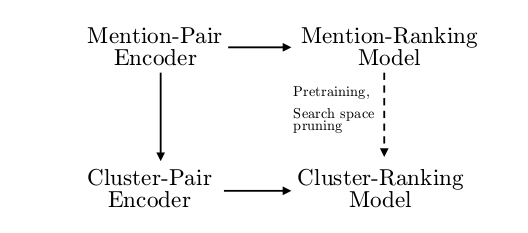
\includegraphics[width=8cm]{deepneural}
\centering
\caption{System Architecture defined in Clark and Mannings 2016 paper.}
\end{figure}

\subsection{Open-Source Implementation}
Though the python source code from \textit{deepcoref} is publically available (Clark and Manning, 2016), it is reliant on StanfordCoreNLP components implemented in Java and is not optimized for speed\footnote{The \textit{deepcoref} system takes roughly 7 days to train on the CoNLL dataset on a GTX Titan GPU.}. For this project, I used the neuralcoref library - an open-source cython library built by \textit{Hugging Face}. Neuralcoref is greatly inspired by Clark/Mannings coreference system. It is SpaCy pipeline extension so it uses SpaCy’s document annotations (which I will discuss in further detail in just a moment). Flexibility regarding SpaCy models and other pipeline components (EntityLinker, EntityRuler, etc.). Neuralcoref ships pretrained on the ConLL 2012 dataset and tuned vectors (word embeddings) trained on the OntoNotes 5.0 dataset.

\section{Dataset and Baseline Evaluation}
To evaluate the performance of this system, I used the annotated coreference resolution dataset from the 2011 BioNLP shared task. The goal of this shared task is to find anaphoric expressions to proteins.The annotated data includes 2,300 pubmed abstracts with corresponding protein and gene annotations as well as coreference cluster annotations. Given that the neuralcoref library evaluates performance based off a file in the tabular CoNLL format, I wrote an evaluation script that closely follows the ‘match’ guidelines outlined in the shared task\footnote{Writing these custom evaluation scripts proved to be quite helpul when investigating why and where the system was performing poorly.}
The system was evaluated using F1, precision, and recall scores. These metrics are calculated by comparing predicted cluster pairs vs. gold annotated cluster pairs. A true postive is counted when a  predicted cluster comprises mentions of which both are either within a minimum span of a gold mention\footnote{Some mentions in the annotated text have a minimum span that \textit{must} be included in the mention span. These minmum spans are generally genes or proteins.} or that a mention subsumes a gold mention of a gold cluster. 

\begin{center}
 \begin{tabular}{||c c c c||} 
 \hline
  &  Prec.  & Rec. & $F1$ \\ [0.5ex] 
 \hline\hline
     SpaCy Web Md & 15.15\% & 8.37\% & 10.72\% \\ 
 \hline
\end{tabular}
\end{center}

\section{Improvements}
So given a baseline performance score and influenced by recent research, I chose to focus on introducing domain-specific named entity recognition (Choi et al., 2014), dependency parsing, word vectors as well as Knowledge Bases or Ontologies to improve performance. Libraries I used to introduce these were:BioWordVec – 200 dimension word vectors trained using Fasttext algorithm on large pubmed corpus
And for Domain-specific NER and dependency parsing, SciSpaCy which provides full SpaCy pipelines trained on biomedical text. 
Regarding word embeddings: NeuralCoref uses static and tuned 50 dimensional word vectors that are used when calculating both  mention embeddings as well as pair embeddings. Given that BioWordVec uses 200 dimensional vectors, I trained a new set of 50 dimensional word vectors on a corpus comprising 1 million Pubmed abstracts and a sampling of random walk sequences from a MeSh graph (Node2Vec).

\section{Results}
Given the high number of False Positives, I chose to improve precision as much as possible to avoid a ‘needle in the haystack’ problem when using this system in an nlp task.

The most performant combination was the use of the SciSpacy model, and pruning using a named entity recognition module trained on the JNLPBA corpus.

We see that in the third row of the table, very poor performance using word vectors trained on biomedical text. This can likely be attributed to the fact that the system was trained using the 50 dimensional google news vectors, so to see any performance gains using domain specific vectors we would need to retrain the system using these vectors.
\begin{center}
 \begin{tabular}{||c c c c||} 
 \hline
  &  Prec.  & Rec. & $F1$ \\ [0.5ex] 
 \hline\hline
     JNLPBA NER & 34.14\% & 11.17\% & 16.83\% \\ 
     SciSpacy MD & 29.86\% & 14.29\% & 19.33\% \\ 
     SciSpacy MD BWV & 2.02\% & 7.27\% & 3.16\% \\ 
 \hline
\end{tabular}
\end{center}
\newpage
\bibliographystyle{plain}
\bibliography{References}

\nocite{pilehvar-collier-2016-improved, choi-etal-2014-analysis, Prokofyev:2015:SOC:2942298.2942337, clark-manning-2016-improving}

\end{document} % end document
